% Source for Fig. 1 — compile with: pdflatex conceptual_model.tex  → conceptual_model.pdf (vector)
\documentclass[tikz,border=4pt]{standalone}
\usepackage[T1]{fontenc}
\usepackage{helvet}\renewcommand{\familydefault}{\sfdefault}
\usetikzlibrary{positioning,shapes.geometric,shapes.symbols,calc,arrows.meta}

\definecolor{t1}{HTML}{F6C94B} % Theme 1 yellow
\definecolor{t1l}{HTML}{FBE9A8}
\definecolor{t2}{HTML}{8ECAC8} % Theme 2 teal
\definecolor{t2l}{HTML}{CDEAE9}
\definecolor{t3}{HTML}{BCD86C} % Theme 3 light green
\definecolor{t3l}{HTML}{E3EFC0}
\definecolor{t4}{HTML}{4CAF50} % Theme 4 green
\definecolor{t4l}{HTML}{BFE3C0}
\definecolor{core}{HTML}{D9D9D9}

\begin{document}
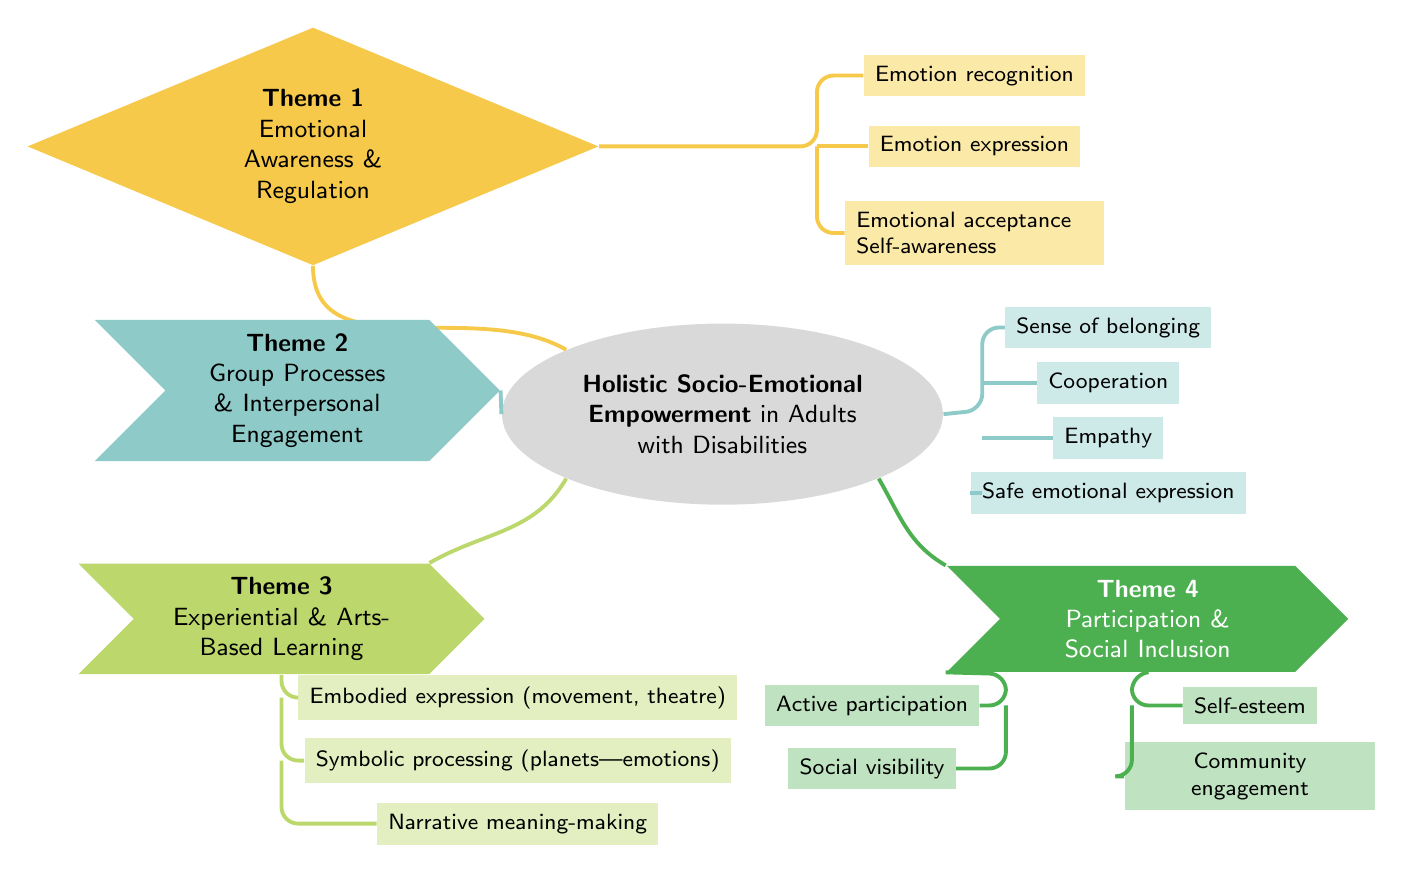
\begin{tikzpicture}[
  font=\small,
  theme/.style={draw=none, text width=3.2cm, align=center, inner sep=5pt, font=\small\bfseries},
  item/.style={draw=none, inner sep=4pt, font=\footnotesize, align=left},
  conn/.style={line width=1.4pt, rounded corners=6pt},
]

% ── Core ─────────────────────────────────────────────────────────
\node[ellipse, fill=core, minimum width=5.6cm, minimum height=2.3cm, align=center] (core) at (0,0)
  {\textbf{Holistic Socio-Emotional}\\\textbf{Empowerment} in Adults\\with Disabilities};

% ── Theme 1 (top-left) ───────────────────────────────────────────
\node[theme, diamond, aspect=2.4, fill=t1, text width=2.6cm] (t1) at (-5.2,3.4)
  {Theme 1\\\normalfont\small Emotional Awareness \& Regulation};
\node[item, fill=t1l] (t1a) at (3.2,4.3) {Emotion recognition};
\node[item, fill=t1l] (t1b) at (3.2,3.4) {Emotion expression};
\node[item, fill=t1l, text width=3.0cm] (t1c) at (3.2,2.3) {Emotional acceptance\\Self-awareness};
\draw[conn, t1] (t1.east) -- (1.2,3.4) -- (1.2,4.3) -- (t1a.west);
\draw[conn, t1] (1.2,3.4) -- (t1b.west);
\draw[conn, t1] (1.2,3.4) -- (1.2,2.3) -- (t1c.west);
\draw[conn, t1] (t1.south) to[out=-90,in=150] (core.north west);

% ── Theme 2 (left) ───────────────────────────────────────────────
\node[theme, fill=t2, shape=signal, signal from=west, signal to=east, text width=3.0cm] (t2) at (-5.4,0.3)
  {Theme 2\\\normalfont\small Group Processes \& Interpersonal Engagement};
\node[item, fill=t2l] (t2a) at (4.9,1.1) {Sense of belonging};
\node[item, fill=t2l] (t2b) at (4.9,0.4) {Cooperation};
\node[item, fill=t2l] (t2c) at (4.9,-0.3) {Empathy};
\node[item, fill=t2l] (t2d) at (4.9,-1.0) {Safe emotional expression};
\draw[conn, t2] (t2.east) -- (core.west);
\draw[conn, t2] (core.east) -- (3.3,0.05) -- (3.3,1.1) -- (t2a.west);
\draw[conn, t2] (3.3,0.4) -- (t2b.west);
\draw[conn, t2] (3.3,-0.3) -- (t2c.west);
\draw[conn, t2] (3.3,-1.0) -- (t2d.west);

% ── Theme 3 (bottom-left) ────────────────────────────────────────
\node[theme, fill=t3, shape=signal, signal from=west, signal to=east, text width=3.4cm] (t3) at (-5.6,-2.6)
  {Theme 3\\\normalfont\small Experiential \& Arts-Based Learning};
\node[item, fill=t3l] (t3a) at (-2.6,-3.6) {Embodied expression (movement, theatre)};
\node[item, fill=t3l] (t3b) at (-2.6,-4.4) {Symbolic processing (planets---emotions)};
\node[item, fill=t3l] (t3c) at (-2.6,-5.2) {Narrative meaning-making};
\draw[conn, t3] (core.south west) to[out=-120,in=30] (t3.north east);
\draw[conn, t3] (t3.south) -- (-5.6,-3.6) -- (t3a.west);
\draw[conn, t3] (-5.6,-3.6) -- (-5.6,-4.4) -- (t3b.west);
\draw[conn, t3] (-5.6,-4.4) -- (-5.6,-5.2) -- (t3c.west);

% ── Theme 4 (bottom-right) ───────────────────────────────────────
\node[theme, fill=t4, text=white, shape=signal, signal from=west, signal to=east, text width=3.4cm] (t4) at (5.4,-2.6)
  {Theme 4\\\normalfont\small Participation \& Social Inclusion};
\node[item, fill=t4l] (t4a) at (1.9,-3.7) {Active participation};
\node[item, fill=t4l] (t4b) at (1.9,-4.5) {Social visibility};
\node[item, fill=t4l] (t4c) at (6.7,-3.7) {Self-esteem};
\node[item, fill=t4l, text width=2.9cm, align=center] (t4d) at (6.7,-4.6) {Community engagement};
\draw[conn, t4] (core.south east) to[out=-60,in=150] (t4.north west);
\draw[conn, t4] (t4.south west) -- (3.6,-3.3) -- (3.6,-3.7) -- (t4a.east);
\draw[conn, t4] (3.6,-3.7) -- (3.6,-4.5) -- (t4b.east);
\draw[conn, t4] (t4.south) -- (5.2,-3.3) -- (5.2,-3.7) -- (t4c.west);
\draw[conn, t4] (5.2,-3.7) -- (5.2,-4.6) -- (t4d.west);

\end{tikzpicture}
\end{document}
